
%% Use the options 1p,twocolumn; 3p; 3p,twocolumn; 5p; or 5p,twocolumn
%% for a journal layout:
 \documentclass[final,1p,times]{elsarticle}
% \documentclass[final,1p,times,twocolumn]{elsarticle}
%% \documentclass[final,3p,times]{elsarticle}
%% \documentclass[final,3p,times,twocolumn]{elsarticle}
%% \documentclass[final,5p,times]{elsarticle}
%% \documentclass[final,5p,times,twocolumn]{elsarticle}

\usepackage{graphicx}
\usepackage{amssymb}
\usepackage{amsthm}
\usepackage{amsmath}

%% Macros
\def\trainingset{\{x_i,y_i\}_{i=0}^{N-1}}
\def\pnmlSingle{\max_{\theta} P_\theta (y_N|x_N, z^N)}

\journal{...}
\begin{document}
\begin{frontmatter}

%% Title, authors and addresses
\title{Predictive Normalized Likelihood for Regression}

%% use the tnoteref command within \title for footnotes;
%% use the tnotetext command for the associated footnote;
%% use the fnref command within \author or \address for footnotes;
%% use the fntext command for the associated footnote;
%% use the corref command within \author for corresponding author footnotes;
%% use the cortext command for the associated footnote;
%% use the ead command for the email address,
%% and the form \ead[url] for the home page:
%%
%% \title{Title\tnoteref{label1}}
%% \tnotetext[label1]{}
%% \author{Name\corref{cor1}\fnref{label2}}
%% \ead{email address}
%% \ead[url]{home page}
%% \fntext[label2]{}
%% \cortext[cor1]{}
%% \address{Address\fnref{label3}}
%% \fntext[label3]{}

%% use optional labels to link authors explicitly to addresses:
%% \author[label1,label2]{<author name>}
%% \address[label1]{<address>}
%% \address[label2]{<address>}

\begin{abstract}
%% Text of abstract

\end{abstract}

\begin{keyword}
Normalized Maximum Likelihood \sep Regression \sep Universal Prediction
\end{keyword}

\end{frontmatter}


%% main text
\section{Introduction} \label{Introduction}
In machine learning the most common tasks are classification and regression. In classification, given train set which consist N pairs $z^N=\{(x_i, y_i)\}_{i=0}^{N-1}$ where $x \in \mathcal{X}$ is the data and $y \in \mathcal{Y}$ are the labels for which $\mathcal{Y}$ is a finite set. The goal is to predict the label $y_N$ of unseen data $x_N$.  The regression task setting are the same as the classification except that the label space $\mathcal{Y}$ is infinite and continuous.
In the general case we estimate the true probability assignment $P(y_N|x_N)$  with the estimator which based on the train set $q(y_N|x_N, z^N)$ . Using the framework of the information theory field our loss is the log-loss
\begin{equation*}
l(q,y_N) = -P(y_N|x_N)\log {q(y_N|x_N})
\end{equation*}The main settings of the way the pairs $\{x,y\}$ are generated are the stochastic setting and individual settings. In the stochastic setting the data and labels are assumed to be generated from probabilistic source, i.e. there is probabilistic assignment $P_\theta(y|x)$ from a set of estimator class $\theta \in \Theta$ and our goal is to find it. In this paper we assume the scenario of the individual setting in which there is not rule of creating the data and labels. Finding assignment of y given x is impossible and therefore we try to be as good as a Jinni which is a learner who has information about the training set along with the label of the test sample and it is constrained to be one of a class of predictors $\{P_\theta(y_N|x_N,y_N,z^N)\ , \ \theta \in \Theta \}$. The log-loss difference between our learner and the Jinny is known as the regret:
\begin{equation}
    R(\theta, q, x_N, z^N) = \sum_{y \in \mathcal{Y}} P_\theta(y_N|x_N,y_N,z^N) log \frac{P_\theta(y_N|x_N,y_N,z^N)}{q_(y_N|x_N, z^N)} 
\end{equation}

The most common approach of generating a leaner is the Empirical Risk Minimization (ERM). Given a training set, a predictor is chosen from a predictors class $\{P_\theta(y|x) , \quad \theta \in \mathcal{\theta}\}$ in a way it minimizes the training set error 
\begin{equation}
    q(y|x) = \min_\theta \frac{1}{N}\sum_{i=0}^{N-1}  l(y_i,P_\theta(y_i|x_i)).
\end{equation}
The underline assumption is that the setting of the problem is the stochastic setting and that training data distribution is as the test data. 

In this paper we use the Predictive Normalized Likelihood (PNML). We assume the label of the test data is known, fit a learner to it and predict the assumes label by it. We repeat the process for all possible label. In the end we normalize the probabilities from each label and return the PNML estimator:
\begin{equation}
    q_{PNML}(y_N|x_N,z^N)=\frac{\pnmlSingle}{\sum_{y\in \mathcal{Y}} \pnmlSingle}
\end{equation}
The paper outline is as follow:
section \ref{sec:FormalProblemDef} describes the setting and the goal of the regression problem. In section \ref{sec:PNMLeval} the evaluation of the PNML is presented and analyses. The simulation of the PNML and its regret on estimating polynomial coefficients is shown in section \ref{sec:Simulation} and the conclusion and future work is in section \ref{sec:Conclusion}.


\section{Formal Problem Definition} \label{sec:FormalProblemDef}
Given data and labels $\{x_i, y_i\}_{i=0}^{N-1}$ where $x_i \in R^M, y\in R$ are deterministic. Our model takes the form:
\begin{equation}
y_i=x_i^T \theta + e_i
\end{equation}
where $\theta \in R^M$ are the learnable parameters and $e$ is white Gaussian noise with variance of $\sigma$. Our goal is to predict $y_N$ based on a new sample $x_N$:
\begin{equation}
y_N = x_N^T \theta + e_N
\end{equation}
In this case $y_N$ has Gaussian distribution which depends on the learnable parameters $\theta$ 
\begin{equation}
P_{\theta}(y_N) 
=\frac{1}{\sqrt[]{2\pi\sigma^2}}exp\bigg\{-\frac{1}{2\sigma^2}\big(y_N- x_N^T\theta \big)^2\bigg\}  \\
\end{equation}
Denote $\Gamma=\int_R \max_{\theta} P_\theta(y_N|X^T)dy_N$ the PNML estimator of $y_N$ given $\{x_i,y_i\}_{i=0}^{N-1}$ and $x_N$ is:
\begin{equation} \label{eq:pnml_def}
q_{PNML}(y_N|x_N,z^N) = \frac{1}{\Gamma} \max_{\theta} P_\theta(y_N)
\end{equation}


\section{PNML Evaluation} \label{sec:PNMLeval}
Using the notations $X = \begin{bmatrix} x_0 & x_1 & \dots & x_N \end{bmatrix}$,
$y = \begin{bmatrix} y_0 & y_1 & \dots & y_N \end{bmatrix} ^T$,
$e = \begin{bmatrix} e_0 & e_1 & \dots & e_N  \end{bmatrix}  ^T$
and assuming that the label of $x_N$ is given ($y_N$ is known), the optimal solution under the mean square error is the least squares estimator:
\begin{equation}
\theta ^*_N = (X^T X)^{-1} X y
\end{equation}
Rewrite it in the recursive least square formulation:
\begin{equation} \label{eq:rls_update}
\theta ^*_N=\theta^*_{N-1} + P_N x_n (x_N^T \theta^*_{N-1} - y_n)
\end{equation}
where $\theta ^*_{N-1}$ is the optimal predictor based on the samples $\{x_i, y_i\}_{i=0}^{N-1}$ and $P_N$ is the covariance matrix of the data. Without loss of generality, when $\mu _{X} = 0$ then $P_N = (XX^T)^{-1}$ 
The probability distribution of our estimation of $y_N$ can be written as
\begin{equation}
\begin{split}
P_{\theta_N ^*}(y_N) 
&=\frac{1}{\sqrt[]{2\pi\sigma^2}}exp\bigg\{-\frac{1}{2\sigma^2}\big(y_N- x_N^T\theta ^*_N \big)^2\bigg\}  \\
&=\frac{1}{\sqrt[]{2\pi\sigma^2}}exp\bigg\{-\frac{1}{2\sigma^2}\bigg(y_N- x_N^T \big(\theta^*_{N-1} + P_N x_N (y_N - x_N^T \theta^*_{N-1}) \big) \bigg)^2\bigg\}  \\
&=\frac{1}{\sqrt[]{2\pi\sigma^2}}
exp\bigg\{-\frac{1}{2\sigma^2}\bigg((1-x_N^T P_N x_N)y_N- x_N^T \theta^*_{N-1} + x_N^T P_N x_N x_N^T \theta^*_{N-1} \bigg)^2\bigg\}  \\
&=\frac{1}{\sqrt[]{2\pi\sigma^2}}
exp\bigg\{-\frac{1}{2\sigma^2}\bigg((1-x_N^T P_N x_N)y_N-(1 - x_N^T P_N x_N ) x_N^T \theta^*_{N-1} \bigg)^2\bigg\}  \\
&=\frac{1}{\sqrt[]{2\pi\sigma^2}}
exp\bigg\{-\frac{(1 - x_N^T P_N x_N )^2 }{2\sigma^2}\bigg(y_N-x_N^T \theta^*_{N-1} \bigg)^2\bigg\}  \\
\end{split}
\end{equation}


Evaluation of the PNML normalization factor from eq. \ref{eq:pnml_def}  gives:
\begin{equation}
\begin{split}
\Gamma &=\int_R \max_{\theta} P_\theta(y_N|X^T)dy_N =\int_{-\infty}^{\infty} \frac{1}{\sqrt[]{2\pi\sigma^2}}
exp\bigg\{-\underbrace{\frac{(1 - x_N^T P_N x_N )^2 }{2\sigma^2}}_{c^2}
\bigg(y_N-\underbrace{x_N^T \theta^*_{N-1}}_{b}\bigg)^2\bigg\} dy_N\\ 
&=\int_{-\infty}^{\infty} \frac{1}{\sqrt[]{2\pi\sigma^2}}
exp\{-c^2\big(y_N-b\big)^2\} dy_N 
=\frac{1}{\sqrt[]{2\pi\sigma^2}} \frac{\sqrt[]{\pi}}{c} 
=\frac{1}{\sqrt[]{2\pi\sigma^2}} \frac{\sqrt[]{\pi}}{\sqrt[]{\frac{(1 - x_N^T P_N x_N )^2 }{2\sigma^2}}}  \\
&=\frac{1}{1 - x_N^T P_N x_N } 
=\frac{1}{1 - x_N^T (XX^T)^{-1} x_N } \\
\end{split}
\end{equation}

% For the 1D estimator case $X=[x_1,\dots,x_N]$
% \begin{equation}
% \Gamma = \frac{1}{1-x_N \frac{1}{\sum_{i=0}^N x_i^2} x_N}
% =\frac{\sum_{i=0}^N x_i^2}{\sum_{i=0}^N x_i^2-x^2_N } =\frac{\sum_{i=0}^N x_i^2}{\sum_{i=0}^{N-1} x_i^2} = 1+ \frac{x_N^2}{\sum_{i=0}^{N-1} x_i^2}
% \end{equation}
% which is the same as \ref{NormalizationNDim}
And finally, given a new data sample $x_N$ the PNML of $y_N$ is:
\begin{equation}
q_{PNML}(y_N)
&=\frac{1}{\Gamma}\max_{\theta}P_{\theta}(y_N) \\
&=\frac{1 - x_N^T (XX^T)^{-1} x_N }{\sqrt[]{2\pi\sigma^2}}
exp\bigg\{-\frac{(1 - x_N^T (XX^T)^{-1} x_N )^2 }{2\sigma^2}\bigg(y_N-x_N^T \theta^*_{N-1} \bigg)^2\bigg\} \\
\end{equation}


We can also calculate the regret of the PNML which is the log of the normalization factor:
\begin{equation} \label{eq:regret}
% \begin{split}
log(\Gamma)
&=log\left(\frac{1}{1 - x_N^T (XX^T)^{-1} x_N } \right) \\
&= -log(1 - x_N^T (XX^T)^{-1} x_N) 
% \end{split}
\end{equation}

\section{PNML with Regularization} \label{sec:PNMLwithReg}
The previous section dealt with the least squares estimator. Here we show the evaluation in case of the least squares with regularization term
\begin{equation}
    Loss(X,y)= ||y-X^T \theta||_2 + \lambda ||\theta||_2
\end{equation}
where $\lambda$ is the regularization term.
In this case the solution of the estimator is
\begin{equation}
\theta ^*_N = (X^T X+ \lambda I)^{-1} X y
\end{equation}
Rewrite it in the recursive least square formulation 
\begin{equation}
\theta ^*_N=\theta^*_{N-1} + P_N x_n (x_N^T \theta^*_{N-1} - y_n)
\end{equation}
which is the same as Equation \ref{eq:rls_update}, however, in this case $P_N= (X^T X+ \lambda I)$. The rest of the PNML evaluation stays the same and therefore the normalization factor becomes
\begin{equation}
    \Gamma =\frac{1}{1 - x_N^T (XX^T+ \lambda I)^{-1} x_N } 
\end{equation}
and the predictor is 
\begin{equation}
q_{PNML}(y_N, \lambda)
&=\frac{1 - x_N^T (XX^T + \lambda I)^{-1} x_N }{\sqrt[]{2\pi\sigma^2}}
exp\bigg\{-\frac{(1 - x_N^T (XX^T + \lambda I)^{-1} x_N )^2 }{2\sigma^2}\bigg(y_N-x_N^T \theta^*_{N-1} \bigg)^2\bigg\} \\
\end{equation}

\section{Simulation} \label{sec:Simulation}
We run a simulation in which we generated uniformly 5 random points in the interval [-1, 1] with zero mean. The goal is to estimate the polynomial coefficient. The least square estimator is shown in Figure \ref{fig:least_sqaures}. we used the PNML estimator and computed its regret from equation \ref{eq:regret} and the it is shown in Figure \ref{fig:regret} 

We run another simulation in which we generated uniformly 10 random points. Then, least squares estimator with regularization was fitted to the generated data. The regularization weight $lambda$ values where 0, 0.1 and 1.0. The least square estimator with the different regularization terms is shown in Figure \ref{fig:least_sqaures_with_reg}. The regret of the PNML estimator with regularization of the same data is in Figure \ref{fig:regret_with_reg} 

\begin{figure}[h] 
\centering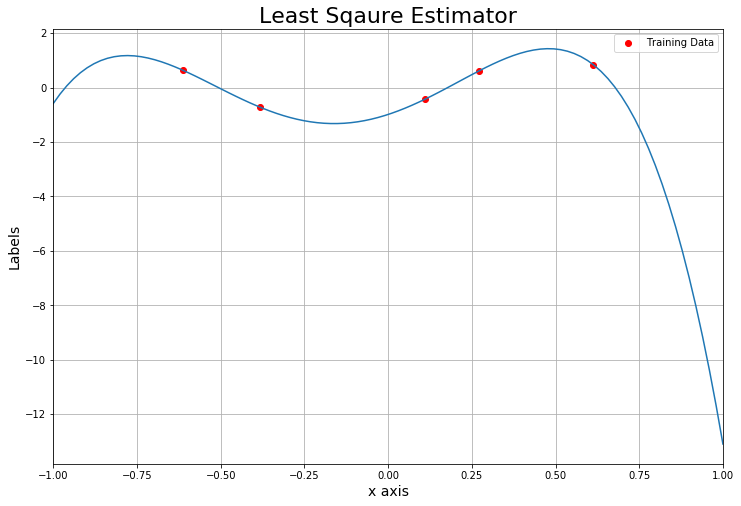
\includegraphics[width=0.6\linewidth]{least_sqaures_plot.png}
\caption{The fitted least square estimator based on the training set.}
\label{fig:least_sqaures}
\end{figure}

\begin{figure}[h]
\centering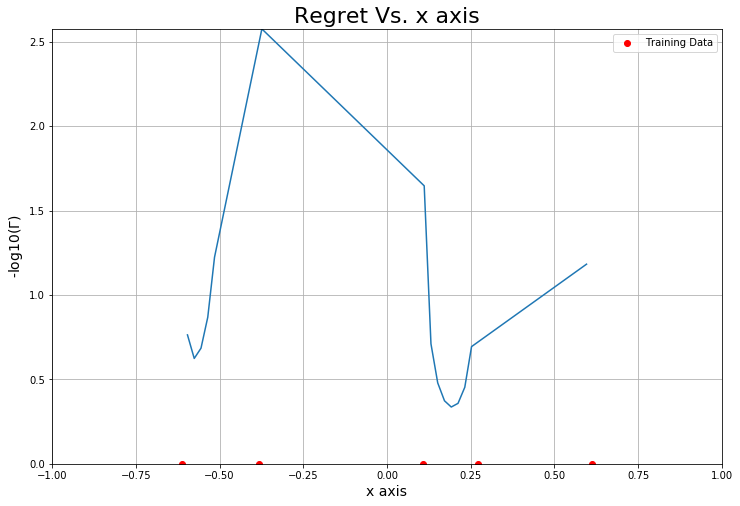
\includegraphics[width=0.6\linewidth]{regret_plot.png}
\caption{The regret of the PNML estimator.}
\label{fig:regret}
\end{figure}

\begin{figure}[h] 
\centering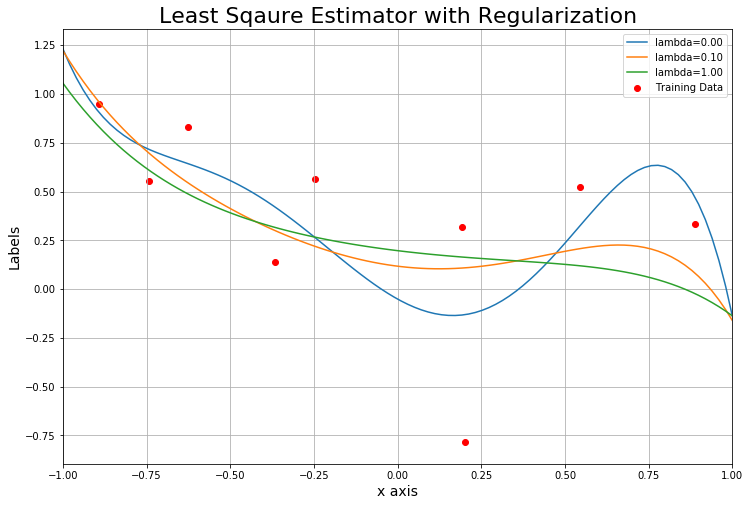
\includegraphics[width=0.6\linewidth]{least_sqaure_with_reg_plot.png}
\caption{The fitted least squares estimator with regularization.}
\label{fig:least_sqaures_with_reg}
\end{figure}

\begin{figure}[h]
\centering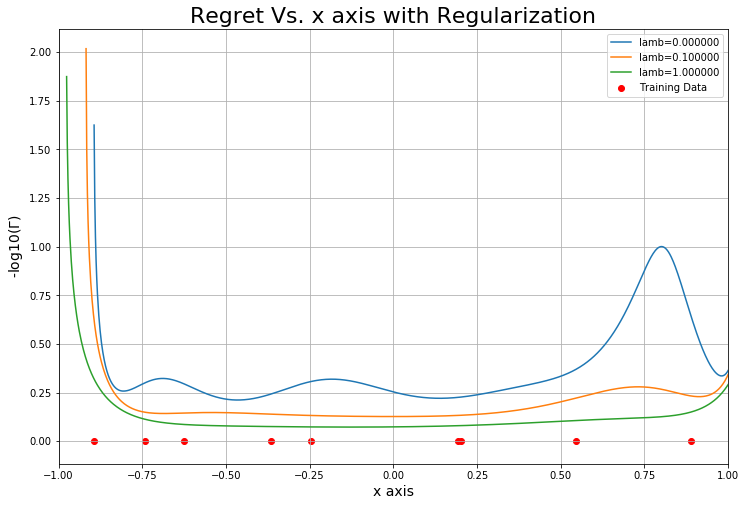
\includegraphics[width=0.6\linewidth]{regret_with_reg_plot.png}
\caption{The regret of the PNML estimator with regularization.}
\label{fig:regret_with_reg}
\end{figure}

\section{Conclusion} \label{sec:Conclusion}
Place holder.



\bibliographystyle{model1-num-names}
\bibliography{references.bib}




\end{document}
